\chapter{Measuring compiler framework performance}
\label{chap:measuring-compiler-performance}

%% Introduction
% Hook
In this chapter, we measure the runtime performance of two user-extensible compiler frameworks: MLIR and xDSL.
% Argument
The usefulness of these measurements are three-fold. First, we provide insight into the current relative performance of MLIR and xDSL. % interesting in its own right, and as a baseline for optimisation
Second, we identify the components of the implementation which contribute most to the overall runtime, and as such are the best targets for optimisation (\autoref{chap:specialising-optimising-pattern-rewriting}) as a corrollary of Amdahl's law \cite{amdahlValiditySingleProcessor1967}.
Finally, we isolate small, self-contained components of the implementation which are comparable between MLIR and xDSL, through which the impact of dynamism can be examined (\autoref{chap:dynamism-pattern-rewriting}).
% Link





\section{Methodology}
\label{sec:methodology}

%% Short intro
% Hook
Accurate performance measurement is a fundamental and notoriously fickle discipline in systems research \cite{}.
% Argument
% Link
In this section, we discuss our methodology for performance measurement, aiming to justify design decisions and facilitate reproducibility

\subsection{Experimental setup}
\label{ssec:experimental-setup}

%% Reproducibility
% Hook
The reproducibility of experiments is critical for a robust scientific methodology.
% Argument
To aid in reproducibility, we provide a description of our experimental setup (\autoref{tab:experimental-setup}).
The choice to use an AWS EC2 instance for performance measurement was partially driven by practical limitations of the resources available to the authors.
This choice incurs a cost
However, there are also commensurate benefits to this choice with respect to reproducibility. This is because researchers aiming to replicate the work can simply create their own EC2 instance with the same configuration, obviating the issue of different hardware configurations affecting performance results.
Furthermore, virtualised systems are representative of real-world workloads
In addition to this, with cloud computing becoming ubiquitous over the past decade, their is a fair body of research into reliable performance measurements on virtualised systems
% Link

\begin{table}[H]
  \caption{Summary of experimental setup configuration used for performance measurement.}
  \label{tab:experimental-setup}
  \centering
  \begin{tabular}{lll}
    \toprule
    \textbf{Configurable} & \textbf{Configuration} \\
    \midrule
    \textit{AWS instance type} & c5a.4xlarge EC2 \\
    \textit{Operating system} & Debian 24.04 (Noble) \\
    \textit{CPU name} & AMD EPYC 7R32 \\
    \textit{Logical CPU cores} & $16$ \\
    \textit{Clock frequency [MHz]} & $2799.99$ \\
    \textit{L1 Data Cache [KiB]} & $32$ \\
    \textit{L1 Instruction Cache [KiB]} & $32$ \\
    \textit{L2 Unified Cache [KiB]} & $512$ \\
    \textit{L3 Unified Cache [KiB]} & $16384$ \\
    \textit{RAM [GB]} & 16 \\
    \bottomrule
  \end{tabular}
\end{table}




\subsection{Experimental configuration}
\label{ssec:experimental-workloads}

% Hook
% Argument
% Link

\begin{table}[H]
  \caption{Summary of experimental setup configuration used for performance measurement.}
  \label{tab:experimental-setup}
  \centering
  \begin{tabular}{lll}
    \toprule
    \textbf{Configurable} & \textbf{Configuration} \\
    \midrule
    \textit{xDSL commit SHA} & \texttt{0eda7fe} \\
    \textit{MLIR commit SHA} & \texttt{6516ae4} \\
    \midrule
    \textit{Python interpreter} & CPython 3.10.17 \\
    \textit{C++ compiler} & clang 18.1.8 \\
    \textit{CMake version} & 3.28.3 \\
    \textit{Ninja version} & 1.11.1 \\
    \bottomrule
  \end{tabular}
\end{table}



\subsection{Experimental workloads}
\label{ssec:experimental-workloads}

% Constant folding
% Hook
% Argument
% Link


\vspace{2em}

\begin{code}
    \begin{minted}{python}
import random

from xdsl.dialects.arith import AddiOp, ConstantOp
from xdsl.dialects.builtin import IntegerAttr, ModuleOp, i32
from xdsl.dialects.test import TestOp
from xdsl.ir import Operation

RANDOM_SEED = 0


def constant_folding_module(size: int) -> ModuleOp:
    """Generate a constant folding workload of a given size."""
    assert size >= 0
    random.seed(RANDOM_SEED)
    ops: list[Operation] = []
    ops.append(ConstantOp(IntegerAttr(random.randint(1, 1000), i32)))
    for i in range(1, size + 1):
        if i % 2 == 0:
            ops.append(AddiOp(ops[i - 1], ops[i - 2]))
        else:
            ops.append(ConstantOp(IntegerAttr(random.randint(1, 1000), i32)))
    ops.append(TestOp([ops[(size // 2) * 2]]))
    return ModuleOp(ops)
    \end{minted}
    \caption{.}
    \label{listing:constant-folding-workload}
\end{code}

\vspace{2em}

% \begin{code}
%    \centering
%     \begin{minted}[fontsize=\footnotesize]{mlir}
% "builtin.module"() ({
%   %0 = "arith.constant"() {"value" = 1 : i32} : () -> i32
%   %1 = "arith.constant"() {"value" = 1 : i32} : () -> i32
%   %2 = "arith.addi"(%1, %0) : (i32, i32) -> i32
%   %3 = "arith.constant"() {"value" = 1 : i32} : () -> i32
%   %4 = "arith.addi"(%3, %2) : (i32, i32) -> i32
%   %5 = "arith.constant"() {"value" = 1 : i32} : () -> i32
%   %6 = "arith.addi"(%5, %4) : (i32, i32) -> i32
%   %7 = "arith.constant"() {"value" = 1 : i32} : () -> i32
%   %8 = "arith.addi"(%7, %6) : (i32, i32) -> i32
%   %9 = "arith.constant"() {"value" = 1 : i32} : () -> i32
%   %10 = "arith.addi"(%9, %8) : (i32, i32) -> i32
%   %11 = "arith.constant"() {"value" = 1 : i32} : () -> i32
%   %12 = "arith.addi"(%11, %10) : (i32, i32) -> i32
%   %13 = "arith.constant"() {"value" = 1 : i32} : () -> i32
%   %14 = "arith.addi"(%13, %12) : (i32, i32) -> i32
%   %15 = "arith.constant"() {"value" = 1 : i32} : () -> i32
%   %16 = "arith.addi"(%15, %14) : (i32, i32) -> i32
%   %17 = "arith.constant"() {"value" = 1 : i32} : () -> i32
%   %18 = "arith.addi"(%17, %16) : (i32, i32) -> i32
%   %19 = "arith.constant"() {"value" = 1 : i32} : () -> i32
%   %20 = "arith.addi"(%19, %18) : (i32, i32) -> i32
%   "test.op"(%20) : (i32) -> ()
% }) : () -> ()
%     \end{minted}
%     \caption{``How Slow is MLIR?'' C++ implementation.}
%     \label{listing:ubenchmark-trait-checks-bench-mlir}
% \end{code}



\subsection{Procedure and infrastructure}
\label{ssec:procedure-infrastructure}

% Steps actually taken

% Stuff we built

%% Corrollary benefits
% Hook
In addition to their usefulness for understanding and optimising compiler performance, these benchmarks provide an opportunity to augment the development process of the xDSL project.
% Argument
Benchmarks can be used to characterise the performance impact of changes to the xDSL codebase, making it easier to avoid unnecessary performance regression.
As such, we provide a command line interface for developers to run the benchmarks, with further functionality which supports a variety of profiling tools.
Furthermore, our benchmarks are constructed to interface with air-speed velocity \cite{michaeldroettboomAirspeedvelocityAsv2025}, a tool which runs benchmarks across repository commits. This information is tracked on the xDSL website \url{https://xdsl.dev/xdsl-bench/}, providing a dashboard for the performance characteristics of xDSL over time.
% Link


















\section{End-to-end benchmarks}

%% Introduction, goals
% Hook
The simplest metric for the performance of a system is its overall runtime.
% Argument
% Link

%% How is MLIR/xDSL split up into pipeline phases
% Hook
One of LLVM's key insights was that compilation can be split into a sequence of discrete steps, avoiding the complex control logic of previous state-of-the-art compilers.
% Argument
As such, compilers having LLVM's pedigree, such as MLIR and xDSL, can be modelled as a pipeline -- parsing the input, applying optimisation transformations, and generating a lowered output (\autoref{}).
This allows us to break down end-to-end benchmarks into components of finer granularity for free.
% Link

%% Figure: pipeline phases

\begin{figure}
    \centering
    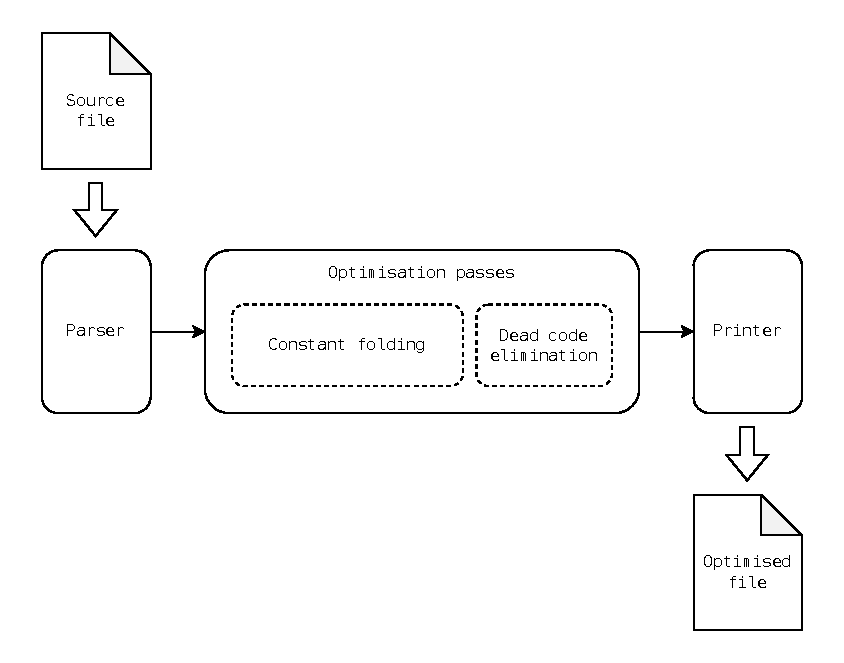
\includegraphics[width=0.75\textwidth]{images/14_measuring_compiler_performance/compiler_phases.drawio.pdf}
    \caption{.}
    % TODO: Does this add value? Could the whole thing be wrapped in an outer box to better communicate the point?
    \label{fig:}
\end{figure}

%% Performance results
% Hook
% Argument
% Link

% Figure: relative performance bar chart
%% Constant folding example. Short but complex example with lots of rewrites?

%% Why pick pattern rewriting?
% Hook
% Argument
% Link







\section{Pattern rewriting}

%% Introduction
% Hook
Having selected pattern rewriting as the compilation phase to examine in detail, we can modify our benchmarks to drive only


% Figure: MLIR vs xDSL across workloads?

% Figure: Trace of MLIR and xDSL overall?








\section{Micro-benchmarks}
\label{sec:ubenchmark}

% Hook
Micro-benchmarking refers measuring the performance of fast, granular, and isolated segments of code.
% Argument
The term was coined by Saavedra et al. in their 1995 paper \cite{saavedraPerformanceCharacterizationOptimizing1995} ``Performance Characterization of Optimizing Compilers''. As such, we are in good company in our application of micro-benchmarking approaches to this problem domain.
Micro-benchmarks have many desirable properties. Since they run quickly, they can cheaply be repeated for statistical confidence.
Furthermore, their fine granularity makes them tractable to reason about -- providing useful information to optimise the component of the system they measure.
However, a key difficulty of micro-benchmarking is ensuring alignment with overall system performance. For example, the selection of code paths to micro-benchmark may introduce bias, making them less representative of the overall system. In addition to this, their performance may be inflated as a consequence of warmed caches and JIT optimisations across repeats, which would not occur during normal operation.
% Link
As such, micro-benchmarking is a useful tool for deeply understanding the performance of software, but must be used carefully to ensure the validity of its results.

% Hook
As discussed in our related work (Section \ref{sec:perf-user-extensible-frameworks}), Amini and Nui's talk ``How Slow is MLIR'' \cite{aminiHowSlowMLIR2024} discusses a set of micro-benchmarks for key operations in the MLIR compiler, such as traversing the IR and creating operations.
% Argument
These micro-benchmarks were used to inform the optimisation of MLIR's data structures and for comparison with traditional LLVM-based compilers. The implementation of the micro-benchmarks allude to an underlying design goal in MLIR by their measurement of asymptotic scaling properties\footnote{\url{https://github.com/joker-eph/llvm-project/blob/6773f827b9ee8055063fcf6b2c6fcdc7f4f579d2/mlir/unittests/Benchmarks/Cloning.cpp\#L66}}. This design goal is asymptotically optimal performance for its underlying data structures. However, data structures with these characteristics often incur constant-time penalties.
This causes overhead for small workloads, where, unlike the asymptotic case, the cost is not amortised. As such, micro-benchmarks may not be representative of the system's overall performance, revealing possibility for the optimisation of code co-designed using them.
Despite this, they can still provide useful insight into MLIR's performance characteristics.
% Link
We implement micro-benchmark workloads for the xDSL equivalent to those for MLIR presented in the keynote, and compare the results of these benchmarks between the two implementations, giving insights into their relative performance.
% We further leverage profiling tools to examine the execution of the two implementations. This allows us to distinguish the cost incurred by the language runtime from the cost incurred by the algorithmic approach of the implementation.

\subsection{Implementation}
\label{ssec:ubenchmark-implementation}

%% Finding and building the MLIR microbenchmarks
% Hook
Unfortunately, the implementation and build instructions for the ``How Slow is MLIR?'' micro-benchmarks were not published with the talk.
% Argument (too informal?)
However, their source code can be found on a branch of the presenter's fork of LLVM\footnote{\url{https://github.com/joker-eph/llvm-project/tree/benchmarks}}. We provide a copy of this source code and instructions for running the benchmarks\footnote{\url{https://github.com/EdmundGoodman/llvm-project-benchmarks}} to enhance the replicability of our results and facilitate further performance experiments.
% Link
This source code can then be used to construct comparable micro-benchmarks in Python.

% Design of our microbenchmarks
% Hook
A key design goal of our micro-benchmarks for xDSL is parity with those provided for MLIR, ensuring the validity their direct comparison.
% Argument
As such, their implementation was derived from the MLIR benchmarks, matching test data and function invocations as closely as possible.
% Link3
In the following sections, we discuss the implementations of a number of micro-benchmarks, facilitating discussion of the insights they give into compiler performance across implementations and language runtimes in later chapters.


\subsection{Operation trait checks}
\label{ssec:ubenchmark-trait-checks}

% Hook
MLIR and xDSL both provide methods to check whether operations have traits.
% Argument
These methods are used very frequently in common tasks. For example, when pattern rewriting over a block of IR, the traits of the block's constituent operations are often used by the matching engine to identify valid rewrites.

% There are two factors which contribute to this slow-down. The first is the inherent overhead incurred by the interpreter loop and data structures in Python's dynamic language runtime. The second is differences in implementation between xDSL and MLIR.
% % Link
% Examining this micro-benchmark in detail allows us to decouple the performance contributions of the implementation and language runtime, and provides insight into the impact of dynamism on user-extensible compiler framework workloads.

\begin{figure}[H]
    \centering
    \begin{subfigure}[b]{0.45\textwidth}
       \centering
        \begin{minted}[fontsize=\footnotesize]{c++}
            // Setup
            Operation op = b.create<OpWithRegion>(
                unknownLoc
            );

            // Benchmark
            bool hasTrait = op->hasTrait<
                OpTrait::SingleBlock
            >();
        \end{minted}
        \caption{``How Slow is MLIR?'' C++ implementation.}
        \label{listing:ubenchmark-trait-checks-bench-mlir}
    \end{subfigure}
    \hfill
    \begin{subfigure}[b]{0.45\textwidth}
        \centering
        \begin{minted}[breakanywhere,fontsize=\footnotesize]{python}
            # Setup
            op = OpWithRegion()

            # Benchmark
            has_trait = op.has_trait(SingleBlock)
        \end{minted}
        \footnotesize\vspace{2em}
        \caption{xDSL Python implementation.}
        \label{listing:ubenchmark-trait-checks-bench-xdsl}
    \end{subfigure}
    \vspace{1em}
    \captionsetup{name=Listing}
    \caption{Micro-benchmark implementations for methods checking an operation has a trait.}
    \label{listing:ubenchmark-trait-checks-bench}
\end{figure}

Micro-benchmarks of checking traits for both implementations (Listing \ref{listing:ubenchmark-trait-checks-bench}) show a slow-down of approximately $130\times$ from MLIR to xDSL (\autoref{tab:ubenchmark-trait-checks}).

\begin{table}[H]
  \caption{Trait checks in xDSL are approximately $130\times$ slower than in MLIR in the asymptotic case.} %, repeated ten times over $32768$ operations. Methodology is discussed in detail in Appendix \ref{} to facilitate replicability.}
  \label{tab:ubenchmark-trait-checks}
  \centering
  \begin{tabular}{cc}
    \toprule
    \textbf{MLIR [ns]} & \textbf{xDSL [ns]}\\
    \midrule
    $3.89 \pm 0.01$ & $504 \pm 76$ \\
    \bottomrule
  \end{tabular}
\end{table}


% % Hook
% The trait checking micro-benchmark yields two key insights.
% % Argument
% The first is that the original implementation of xDSL makes significant tradeoffs of performance for expressivity. By eliminating these tradeoffs, we reveal the Python language runtime incurs a $16\times$ overhead with respect to C++, as a result of the complexity of its evaluation loop.
% The second is that whilst C++ can efficiently represent dynamic functionality, albeit at the cost of implementation complexity, dynamism incurs the cost of obscuring other optimisations that would further widen the performance gap between Python and C++.
% % Link
% However, whilst trait checking is a frequent operation, it alone is not representative of the overall performance of compiler frameworks. As such, further micro-benchmarks and examining representative workloads is required.


\subsection{Operation instantiation}

\subsection{Summary of micro-benchmarks}

% Hook
In addition to the above micro-benchmarks which we examine in detail, we further provide a wider suite of micro-benchmarks discussed in lesser detail for brevity. % The implementations of all xDSL micro-benchmarks are provided in the Appendix (\autoref{}).
% Argument
This suite implements many of the remaining equivalent micro-benchmarks from ``How Slow is MLIR'' (\autoref{tab:ubenchmark-remaining-mlir}).
From these, we can see the trend of a slow-down in the order of $xy\times$ holds

\begin{table}[H]
  \caption{.}
  \label{tab:ubenchmark-remaining-mlir}
  \centering
  \begin{tabular}{ccc}
    \toprule
    \textbf{Benchmark name} & \textbf{MLIR [ns]} & \textbf{xDSL [ns]}\\
    \midrule
    Trait checks & $3.89 \pm 0.01$ & $504 \pm 76$ \\
    ... & ... & ... \\
    \bottomrule
  \end{tabular}
\end{table}


% Hook
In addition to the remaining ``How Slow is MLIR?'' micro-benchmarks, the suite provides further xDSL-only micro-benchmarks sampled from atomic functions invoked by pattern rewriting workloads (\autoref{tab:ubenchmark-xdsl-regression}).
% Argument
These have two-fold use: triaging functions to optimise by longest runtime following Amdhal's law \cite{amdahlValiditySingleProcessor1967}; and serving as a metric of performance to ensure optimisations don't inadvertently introduce regressions.
% Link

% Do a bar chart instead of a table!!!!
% \begin{table}[H]
%   \caption{.}
%   \label{tab:ubenchmark-xdsl-regression}
%   \centering
%   \begin{tabular}{ccc}
%     \toprule
%     \textbf{Benchmark name} & \textbf{xDSL [ns]}\\
%     \midrule
%     Trait checks & $504 \pm 76$ \\
%     ... & ... & ... \\
%     \bottomrule
%   \end{tabular}
% \end{table}
